%
% Project proposal
% Guidelines can be found at: http://courses.cse.tamu.edu/caverlee/csce470/project.html
% 
\documentclass{article}
\renewcommand{\contentsname}{Table of Contents}
\newcommand{\PaperTitle}{Executive Summary}
\usepackage{hyperref}
\usepackage{fullpage}
\usepackage{graphicx}
\usepackage{wrapfig}

%\hypersetup{colorlinks=false}

\begin{document}

%
% Title Page
\newcommand{\HRule}{\rule{\linewidth}{0.5mm}}
%
% Title Page
%
\begin{titlepage}
  \begin{center}
  % Title
  \textsc{\Large FootTraffic}\\[0.5cm]
  \HRule \\[0.4cm]
  {\huge \bfseries \PaperTitle}\\[0.2cm]
  \HRule \\[1cm]
  
  \large{Department of Computer Science \& Engineering} \\
  \large{Texas A\&M University} \\[1cm]

  % Authors and emails
  \begin{minipage}{0.4\textwidth}
    \begin{flushleft} \large
    \emph{Authors:}\\
    William \textsc{Chen} \\
    Eric \textsc{Wood}
    \end{flushleft}
  \end{minipage}
  \begin{minipage}{0.4\textwidth}
    \begin{flushright} \large
    \emph{Emails:} \\
    wchen16@cse.tamu.edu\\
    ebw0178@cse.tamu.edu
    \end{flushright}
  \end{minipage}
  \\[1cm]
  \large{\today}
  \vfill
  
  % Bottom of the page
  \end{center}
\end{titlepage}


%
% Document
% Motivation and Related Works
\section{Motivation and Related Works}
We are seeing an increasing amount of location sharing from social services Foursquare, Facebook, Google Latitude, etc.,
and we want to harness these traffic to recommend venues to users based on the traffic patterns. Most location-based
search engines today rank results based on proximity, user rating, category, and popularity. We want to add another 
dimension to location-based searches, and that is ranking based on observed traffic similarities.
This ``\textit{temporal dynamics embedded in the checkins} from location sharing services''
\footnote{``\href{http://faculty.cs.tamu.edu/caverlee/pubs/cheng11cikm.pdf}{Toward Traffic-Driven Location-Based Web Search}''
  by Zhiyuan Cheng, James Caverlee, Krishna Y. Kamath, and Kyumin Lee; CIKM 2011},
approach is introduced by a research paper authored by Zhiyuan Cheng, James Caverlee, Krishna Y. Kamath,
and Kyumin Lee, and the foundation of FootTraffic search engine will be based on the ideas from the paper
\footnote{A copy of the paper can be found at: \url{http://faculty.cs.tamu.edu/caverlee/pubs/cheng11cikm.pdf}}
aforementioned.

\section{Our Approach}
\begin{wrapfigure}{r}{6cm}
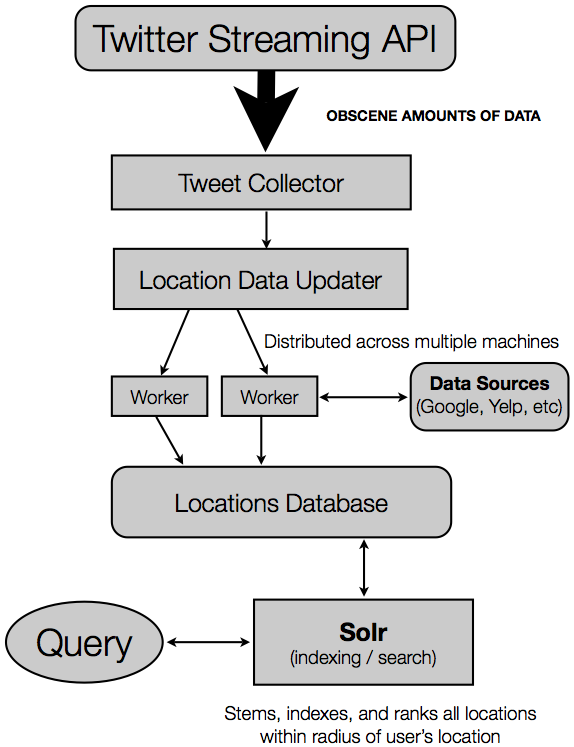
\includegraphics[width=6cm]{flowchart.png}
\caption{Workflow}
\end{wrapfigure}
We have put in a lot of thought into creating efficient and optimized ways of gathering, storing, and serving data. The final solution
we came up with is outlined in the flowchart shown to the right. In the backend, we have scripts, an Apache server with Phusion Passenger
to run Ruby on Rails, a \href{http://lucene.apache.org/solr/}{Solr} instance, and a Postgres database server. In the frontend, we used
a couple Javascript libraries and APIs, such as JQuery, Google Fonts, Google Maps, flot, to handle events and transitions. 
\\ \\
We have two Ruby scripts that are run continuously and concurrently. One is responsible for keeping a connection open with Twitter's realtime
search API, filtering for FourSquare tweets, and inserting an entry to a database table (Checkins). The other is responsible for processing
entries in the Checkins table, then requesting information from Yelp and Google. If the venue already exists in our database, no additional
API calls are made, and the traffic data is updated in the Locations database table. 
\\ \\
Apache, Phusion Passenger, and Ruby on Rails serve the HTTP requests coming from users. When the user makes a query, Rails passes the query
string to Solr, which does the full-text indexing, geospatial and weighted search, and returns the relevant results back to the user.
More information on the weighting will be highlighted in the next subsection.

\subsection{Ranking}
There are a variety of factors that is taken into account when we do ranking, which is all taken care of by Solr. With Solr, we can do a
decent job searching based on names, categories and other metadata. We assigned weightings to the different fields; we toyed with
each until we had overall results which were deemed relevant. In the end we weight the location's name and address the highest, followed 
by the category and then tags which we pulled from Yelp. Rating from Yelp reviews also play a role in determining the final weighting.
In addition Solr indexes geographic coordinates for each location. We can issue
queries with the user's location and specify a precision to limit the results to within a certain geographic range.
%\\ \\
%When a user searches, we retrieve the initial results from Solr, which are then augmented by our own algorithm to take additional factors into account. We take Solr's scores from our query and apply a few procedures on them. The "rating" of a location is important for places such as restaurants, and we take this into account by multiplying the rating (a value between 1 and 5, given to us by Google Places) and a damping factor (0.3 in the final product) and multiplying the result by the Solr score. This has a few disadvantages, as places without scores aren't necessarily going to be ranked as highly. In our tests, however, we determined that other factors made up for this effect and that even relevant places without scores could find their way to the top.
\\ \\
There are two choices for weighting: either the user wants to see popular places, or they want places that are less crowded. When looking 
for popular places, we take into account how popular that specific time is compared to the overall traffic pattern. This is important due
to our dataset not being complete, as results which have more data are more likely to appear over ones that aren't as complete and therefore
aren't as reliable. The final formula used for popular locations is as follows:
\\ \\
\verb|score = score * (10 * (t_pattern_score / t_pattern_max_score))|
\\ \\
The weighting for queries involving less crowded locations is less complicated; we simply subtract 1 from the traffic patterns at that specific time and multiply it by the score.
\\ \\
Finally, we take distance into account when weighting the results. We take the distance and multiply it by a damping factor (0.1 in this case) and then divide the score by it. The result does a decent job in our tests of making sure locations closer to the user are more likely to appear.

\section{Challenges}
One of the largest challenges we faced in this project were accumulating data and storing it in an accessible manner. Since we rely heavily
on external APIs for collecting metadata on our locations, there were numerous API limits placed on us. Google Places has a quota of 1000 queries
per day, and Yelp is extremely limiting. We violated Google and Yelp's terms of service, specifically we stored the data gathered from them. 
If this were to be expanded beyond just an academic exercise, then our data collection would need to be done by crawling websites and determining
tags and relevant data ourselves, as no API we could find would give us the data we needed without placing numerous restrictions on us. After several
weeks of pulling data on a regular basis, several of our worker processes were banned from Yelp, as they (correctly) determined our usage
patterns mirrored those of a bot rather than a real user.
%\\ \\
%The architecture of the application took a considerable amount of effort. From the start of the project we wanted to keep scalability in mind, as a data-driven application has to deal with large quantities of data and requests. We decided to use "delayed\_job," a queuing system that allows for "jobs" to be created and stored in a database which worker processes can then pick up and execute. Since we were going to be splitting the job of processing tweets and pulling in data from APIs across multiple computers, we needed a common database. We decided on PostgreSQL, as it is very well-supported and simple to set up, as well as trusted for large data sets. We wrote a series of jobs that pull checkins from the database and process them, kicking off additional jobs for populating newly created locations with data from Yelp and Google. The results were great, as the system could be administered from a single computer and we could expand to accept larger amounts of data.

\section{Interesting Aspect}
Ranking posed a significant challenge. It took a lot of tweaking to get the weighting on the fields right. Early on in development, results for the
search term ``starbucks'' would show other coffee shops as top results. It turns out that users on Yelp had been comparing local coffee shops to
Starbucks, resulting in a tag weighting that overshadowed the name field. Determining which fields were more relevant to queries took a lot of
experimentation; users aren't always searching for the same parameters, and having a search feature that allows for multiple categories of queries
makes weighting names versus genres difficult. Placing too much emphasis on the location name puts coffee shops with ``coffee'' in the name higher
on the results list for a query for ``coffee''.

\section{Evaluation}
Overall, we're very pleased with our results; not only have we collected a large amount of data, our search results are relevant and useful from the evaluations we've done. We just wish there were more data in College Station! There are a number of user interface improvements that could be made which time didn't allow for. Our search algorithm could use some tweaking and testing with a larger audience. Our capabilities are limited by our dataset, however, and we're very interested in expanding the methods used to collect data, which is a very different information retrieval problem. Weaning ourselves off of external APIs and expanding the number of machines we have processing data would drastically improve our application's usefulness, as we would be able to process much larger amounts of data.

\end{document}
